% ============================================================
% dean-journal-scan.tex: 10-minute journal scan of
%   D. S. Dean, J. Phys. A: Math. Gen. 29, L613 (1996)
% with remarks on follow-up papers.
%
% Look and colour code as in slides2.tex (plain beamer, 12pt):
%   blue = interactions, green = noise, orange = Ito term / entropy.
% Every frame carries a \note{} with what to say; [m:ss] = time for the frame.
% Statements about follow-ups are taken from the PDFs in ../literature/.
%
% Build (from slides/):
%   latexmk -pdf -outdir=.tmp dean-journal-scan.tex        && cp .tmp/dean-journal-scan.pdf .
%   latexmk -pdf -outdir=.tmp dean-journal-scan-notes.tex  && cp .tmp/dean-journal-scan-notes.pdf .
% The second one puts the notes on a second screen (right half of each page).
% ============================================================
\documentclass[12pt,aspectratio=169]{beamer}

\usepackage{amsmath,amssymb}
\usepackage{graphicx}
\usepackage[english]{babel}
\usepackage{cancel}
\usepackage{textcomp}
\usepackage{silence}
\usepackage{catchfile}
\usepackage{ifthen}
\usepackage{animate}
\usepackage{tikz}
\usetikzlibrary{arrows.meta,decorations.pathmorphing,positioning,calc}
\usepackage{pgfpages}
\usepackage{appendixnumberbeamer}

\usepackage{mathtools}
\mathtoolsset{showonlyrefs}



\renewcommand{\CancelColor}{\color{red}} %change cancel color to red

\makeatletter
\let\my@cancelto\cancelto %copy over the original cancelto command
\newcommand<>{\cancelto}[2]{\alt#3{\my@cancelto{#1}{#2}}{\mathrlap{#2}\phantom{\my@cancelto{#1}{#2}}}}
% redefine the cancelto command, using \phantom to assure that the
% result doesn't wiggle up and down with and without the arrow
\makeatother



\newenvironment{wide}[1]{\begin{columns}\column{\dimexpr\paperwidth-#1}}{\end{columns}}

\newenvironment{wide2}[2][1ex]{\begin{columns}\column{\dimexpr\paperwidth-#2}
\begin{minipage}[t][\textheight-#1]{\textwidth}
}{\end{minipage}\end{columns}}


% \definecolor{beamer@blendedblue}{rgb}{0.07,0.20,0.47}
% \setbeamercolor{structure}{fg=beamer@blendedblue}

\definecolor{bblue}{rgb}{0.2,0.2,0.7} % beamer blue
\definecolor{darkred}{rgb}{0.8,0,0}
\definecolor{litered}{rgb}{0.2,1,1}
\definecolor{Darkred}{rgb}{0.7,0,0}
\definecolor{liteyellow}{rgb}{1,1,0.7}
\definecolor{litegreen}{rgb}{0.8,1,0.8}
\definecolor{darkgreen}{rgb}{0,0.5,0}
\definecolor{litelitegray}{rgb}{0.8,0.8,0.8}
\definecolor{litegray}{rgb}{0.6,0.6,0.6}
\definecolor{purple}{rgb}{0.58,0,0.58}
\definecolor{darkmag}{rgb}{0.5,0.0,0.5}
\definecolor{darkorange}{rgb}{0.68,0.28,0.04}
\definecolor{darkbrown}{rgb}{0.55,0.35,0.15}





\newcommand<>{\altfixed}[2]{\alt#3{#1}{\mathrlap{#2}\phantom{#1}}}
\newcommand<>{\altfixedother}[2]{\alt#3{\mathrlap{#1}\phantom{#2}}{#2}}



\renewcommand<>{\mathcolorboxalt}[2]{
	\altfixed#3{{ \setlength{\fboxsep}{0pt} \colorbox{#1}{$\displaystyle #2$}}}{#2}
}




\renewcommand<>\hlbox[2]{%
  \alt#3{\colorbox{#1}{#2}}%
  {\makebox[\dimexpr\width+2\fboxsep]{#2}\vphantom{\colorbox{#1}{#2}}}%
}
\newcommand<>{\mathhlbox}[2]{%
	\alt#3{\colorbox{#1}{$\displaystyle #2$}}%
	{\makebox[\dimexpr\width+2\fboxsep]{$\displaystyle #2$}\vphantom{\colorbox{#1}{$\displaystyle #2$}}}%
}
\newcommand<>{\mathhlboxRGB}[2]{%
	\alt#3{\colorbox[RGB]{#1}{$\displaystyle #2$}}%
	{\makebox[\dimexpr\width+2\fboxsep]{$\displaystyle #2$}\vphantom{\colorbox[RGB]{#1}{$\displaystyle #2$}}}%
}
\newcommand<>{\hlboxRGB}[2]{%
	\alt#3{\colorbox[RGB]{#1}{#2}}%
	{\makebox[\dimexpr\width+2\fboxsep]{#2}\vphantom{\colorbox[RGB]{#1}{#2}}}%
}

\newcommand<>{\mathcolorbox}[2]{
	\alt#3{\colorbox{#1}{$\displaystyle #2$}}{\colorbox{white}{$\displaystyle #2$}}%
}
\newcommand<>{\mathcolorboxRGB}[2]{
	\alt#3{\colorbox[RGB]{#1}{$\displaystyle #2$}}{\colorbox{white}{$\displaystyle #2$}}%
}

\newcommand<>{\mathaltcolorbox}[3]{% color, expr1, expr2 
	\altfixed#4{\colorbox{#1}{$\displaystyle #2$}}{\colorbox{white}{$\displaystyle #3$}}%
}

% define backslash symbol $/$
\newcommand{\bsh}[0]{\textbackslash}




% hide navigation symbols
\setbeamertemplate{navigation symbols}{}
\addtobeamertemplate{navigation symbols}{}{%
	\usebeamerfont{footline}%
	\usebeamercolor[fg]{footline}%
	\hspace{1em}%
	\insertframenumber/\inserttotalframenumber
}

% make boxes rounded
\setbeamertemplate{blocks}[rounded][shadow=false]



% footnote without number
\addtobeamertemplate{footnote}{\hskip -2em}{}
\newcommand{\footnotetextrelaxed}[1]{{\let\thefootnote\relax\footnotetext{#1}}}


\usepackage{catchfile}


% \usepackage{catchfile}
% make animate work in Texpad compiler
\CatchFileDef{\CompilationMode}{mode.txt}{}
\ifthenelse{\equal{\CompilationMode}{make }}{}{
    \renewcommand{\animategraphics}[5][]{\ErrorsOff[xkeyval]\ErrorsOff[keyval]\includegraphics[#1]{#3#4}}
    }


\let\x\relax
% ============================================================
% definitions.tex — macros for manuscript.tex
%
% Carried over from the top-level derivation log (../definitions.tex),
% trimmed of nothing, plus a small block of new macros at the end for
% symbols introduced in the Extrusion/Nucleation section (dean.tex
% "Extrusion rate": Virtual work, The nucleation threshold, Layering
% probability) that did not exist when the derivation-log definitions
% file was written. Keep the two files in sync by hand — there is no
% automated check.
% ============================================================

\newcommand{\la}{\left\langle}
\newcommand{\ra}{\right\rangle}
\newcommand{\bs}{\boldsymbol}
\newcommand{\E}{\mathbf{E}}
\newcommand{\Var}{\text{Var}}
\renewcommand{\d}{\mathrm{d}}
\renewcommand{\u}{\bs{u}}
\newcommand{\q}{\bs{q}}
\newcommand{\Q}{\mathbf{Q}}
\newcommand{\R}{\mathbb{R}}
\newcommand{\n}{\bs{n}}
\newcommand{\e}{\bs{e}}
\newcommand{\T}[0]{\mathrm{T}}
\newcommand{\pd}[2]{\frac{\partial #1}{\partial #2}}
\newcommand{\tpd}[2]{\tfrac{\partial #1}{\partial #2}}


\newcommand{\ab}{{\alpha\beta}}
\newcommand{\mn}{{\mu\nu}}
\newcommand{\abmn}{{\alpha\beta\mu\nu}}

\newcommand{\eye}{\bs{\mathrm{I}}}
\renewcommand{\v}{\mathbf{v}}
\newcommand{\x}{\mathbf{x}}
\newcommand{\f}{\mathbf{f}}
\newcommand{\s}{\mathbf{s}}
\newcommand{\g}{\mathbf{g}}
\newcommand{\G}{\mathbf{G}}
\renewcommand{\H}{\mathbf{H}}
\newcommand{\Ha}{\mathbf{H}_\text{a}}
\newcommand{\F}{\mathbf{F}}
\newcommand{\I}{\mathbf{I}}
\newcommand{\J}{\mathbf{J}}
\newcommand{\bnabla}{\boldsymbol{\nabla}}
\newcommand{\A}{\mathbf{A}}
\newcommand{\B}{\mathbf{B}}
\newcommand{\U}{\mathbf{U}}
\newcommand{\bxi}{\mathbf{\xi}}
\newcommand{\p}{\mathbf{p}}
\newcommand{\W}{\mathbf{W}}
\newcommand{\bT}{\mathbf{T}}
\newcommand{\nh}{\hat{\bs{n}}}
\newcommand{\bdelta}{\bs\delta}
\newcommand{\bsigma}{\bs\sigma}
\newcommand{\bEta}{\bs\eta}
\newcommand{\fa}{\bs{f}_\text{a}}
\renewcommand{\ss}{\mathrm{ss}}

\newcommand{\ee}{\mathrm{e}}
\newcommand{\ii}{\mathrm{i}}

\renewcommand{\k}{\bs{k}}
\renewcommand{\r}{\mathbf{r}}

\newcommand{\TT}{{\rm T}}
\newcommand{\Tr}{{\rm T}}


\newcommand{\lM}{l_{\rm M}}
\newcommand{\lm}{l_{\rm m}}

\newcommand{\elln}{\ell_{\rm n}}
\newcommand{\ellc}{\ell_{\rm c}}
\newcommand{\elld}{\ell_{\rm d}}

\newcommand{\calN}{\mathcal{N}}
\newcommand{\calF}{\mathcal{F}}
\newcommand{\calG}{\mathcal{G}}
\newcommand{\calK}{\mathcal{K}}
\newcommand{\calP}{\mathcal{P}}
\newcommand{\rmR}{\mathrm{R}}

\providecommand{\Fpair}{\calF_{\mathrm{pair}}}
\providecommand{\Fent}{\calF_{\mathrm{ent}}}
\providecommand{\Tr}{\operatorname{tr}}
\newcommand{\frev}{f_{\rm rev}}
\newcommand{\xir}{\xi_{\rm r}}
\newcommand{\ecrit}{\varepsilon_{\rm c}}
\newcommand{\sigmarho}{\sigma_\rho^2}
\newcommand{\kB}{k_\mathrm{B}}
% Correction / open-question annotations (visible in the compiled PDF —
% useful while this is still a skeleton; strip before submission)
\newcommand{\corr}[1]{\textcolor{red}{\textbf{[CORR:}\ #1\textbf{]}}}
\newcommand{\corrm}[1]{{\color{red}#1}}
\newcommand{\todo}[1]{\textcolor{purple}{\textbf{[TODO:}\ #1\textbf{]}}}

\renewcommand{\div}{\text{div}}

\newcommand{\pade}{\text{Pad\'{e}}}
\newcommand{\cell}{\text{cell}}
\newcommand{\crit}{\text{crit}}

\newcommand{\Pa}{\text{Pa}}
\newcommand{\kPa}{\text{kPa}}

\newcommand{\minute}{\text{min}}
\newcommand{\micron}{\upmu\mathrm{m}}
\newcommand{\tcdot}{\!\cdot\!}

\newcommand{\ash}[1]{\textcolor{blue}{\textbf{[ash:}\ #1\textbf{]}}}

% ------------------------------------------------------------
% New in manuscript.tex: symbols from dean.tex's "Extrusion rate"
% section (Virtual work / The nucleation threshold / Layering
% probability), which post-date the derivation-log definitions.tex.
% ------------------------------------------------------------

\newcommand{\gammaw}{\gamma_{\rm w}}           % water/interfacial surface tension (NOT the nematic relaxation rate \gamma, NOT gamma_0 = B/xi_0 — three distinct gammas in this project, see canonical-model-parameters memory)
\newcommand{\Wc}{W_{\rm c}}                    % cell-cell adhesion energy
\newcommand{\Ws}{W_{\rm s}}                    % cell-substrate adhesion energy
\newcommand{\Acell}{A_{\rm cell}}              % single-cell area
\newcommand{\pcrit}{p_{\rm crit}}              % critical pressure, boxed result eq:pcrit
\newcommand{\nuzero}{\nu_0}                    % peak variance modulation, sec-layering-probability
\newcommand{\ellA}{\ell_A}                     % nucleus smoothing scale (superseded alternative — see FRIDGE/fluctuation_mechanism.tex; kept only in case it resurfaces)


% prompt, address all the prompts in the text
\newcommand{\prompt}[1]{\textcolor{blue!90!black}{[ #1 ]}}
\newcommand{\unclear}[1]{{\color{blue}[\textit{unclear}} #1{\color{blue}]}}


\ifdefined\shownotes
  \setbeameroption{show notes on second screen=right}
\fi
\setbeamertemplate{note page}[plain]
\setbeamerfont{note page}{size=\small}
\addtobeamertemplate{note page}{\setlength{\parskip}{0.8ex}}{}
\newcommand{\clk}{\textbf{\textcolor{red}{[click]}}\ }

% ---------------------------------------------------------------------------
% colour code (as in slides2.tex)
\newcommand{\colI}[1]{{\color{bblue}#1}}
\newcommand{\colN}[1]{{\color{darkgreen}#1}}
\newcommand{\colD}[1]{{\color{darkorange}#1}}
\newcommand{\hlf}[1]{{\setlength{\fboxsep}{1pt}\colorbox{liteyellow}{$#1$}}}
\newcommand{\lab}[2]{\underbrace{#1}_{\mathclap{\text{\scriptsize #2}}}}
\newcommand{\deanlegend}{\hfill{\footnotesize \colI{interactions}\quad \colN{noise}\quad \colD{It\^o term}}}
% equation number of the paper, printed next to a display
\newcommand{\eqn}[1]{\text{\scriptsize\color{softgray}(#1)}}
\newcommand{\eqtag}[1]{\tag*{\eqn{#1}}}
% short reference tag
\newcommand{\refs}[1]{{\scriptsize\color{softgray}#1}}
\definecolor{softgray}{rgb}{0.35,0.35,0.35}  % readable grey for content
% follow-up strands
\definecolor{laneD}{rgb}{0.50,0.10,0.55}   % averaged / DDFT
\definecolor{laneS}{rgb}{0.55,0.35,0.15}   % solutions / applications
\definecolor{laneA}{rgb}{0.75,0.05,0.05}   % active matter
\definecolor{laneM}{rgb}{0.00,0.45,0.45}   % mathematics
\tikzset{>={Stealth[length=2.5mm]},
  % styles with a colour argument live here: a # inside a frame body breaks beamer
  card/.style={draw=#1,fill=#1!7,rounded corners=2pt,inner sep=2pt,
               font=\footnotesize,align=center,text width=3.95cm,minimum height=1.15cm},
  lane/.style={font=\footnotesize\bfseries,text=#1,anchor=west},
  box/.style={draw=#1,thick,rounded corners=3pt,fill=#1!6,text width=4.3cm,
              align=left,inner sep=5pt,font=\footnotesize,minimum height=3.3cm,anchor=north},
  num/.style={circle,fill=#1,text=white,font=\bfseries,minimum size=0.8cm,inner sep=0pt},
  txt/.style={anchor=west,align=left,text width=11.3cm},
  % overlay-aware visibility (keeps the layout fixed)
  invisible/.style={opacity=0,text opacity=0},
  alt/.code args={<#1>#2#3}{\alt<#1>{\pgfkeysalso{#2}}{\pgfkeysalso{#3}}},
  visible on/.style={alt={#1{}{invisible}}}}
% density profile used in the pictures: two bumps with an empty gap
\pgfmathdeclarefunction{rhoprof}{1}{\pgfmathparse{exp(-((#1-0.9)/0.45)^2)+0.85*exp(-((#1-3.1)/0.42)^2)}}
% ---------------------------------------------------------------------------

\title{Langevin equation for the density of a system of interacting Langevin processes}
\author{Ashot Matevosyan}
\date{November 2, 2026}

\begin{document}

% ===========================================================================
% 1. The paper
% ===========================================================================
\begin{frame}[plain]
\begin{columns}[c,totalwidth=0.94\paperwidth]
\column{0.66\paperwidth}
\centering
\begin{tikzpicture}
  % page L613 is US letter (612 x 792 pt); crop = title to end of abstract
  \node[anchor=south west,inner sep=0pt] (img) at (0,0)
    {\includegraphics[page=2,trim=62 456 159 45,clip,height=0.86\paperheight]{media/dean1996}};
  \draw[litelitegray] (img.south west) rectangle (img.north east);
  \only<2->{
  \begin{scope}[overlay]
    % zoom: abstract only (x 128..453, y 456..546 pt of page L613)
    \node[anchor=south west,inner sep=3pt,fill=white,draw=litegray,line width=0.8pt] at ($(img.south west)+(0.25,-0.4)$)
      {\phantom{\includegraphics[page=2,trim=128 456 159 246,clip,width=0.88\paperwidth]{media/dean1996}}};
    \node[anchor=south west,inner sep=0pt] (zoom) at ($(img.south west)+(0.25,-0.4)+(3pt,3pt)$)
      {\includegraphics[page=2,trim=128 456 159 246,clip,width=0.88\paperwidth]{media/dean1996}};
    \begin{scope}[shift={(zoom.south west)},x={($(zoom.south east)-(zoom.south west)$)},y={($(zoom.north west)-(zoom.south west)$)},blend mode=multiply]
      \fill[liteyellow] (0.254,0.834) rectangle (0.460,0.957); % simple derivation
      \fill[litegreen]  (0.620,0.398) rectangle (0.974,0.501); % not additively but multiplicatively
      \fill[litegreen]  (0.386,0.288) rectangle (0.925,0.391); % density cannot fluctuate ... particles
      \fill[liteyellow] (0.179,0.065) rectangle (0.469,0.181); % coursed grained free energy
    \end{scope}
  \end{scope}}
\end{tikzpicture}
\column{0.27\paperwidth}
\raggedright
{\Large\color{bblue}\textbf{Journal scan}}

\vspace{3ex}
Ashot Matevosyan

{\footnotesize MPI for the Physics of\\ Complex Systems}

\vspace{1ex}
{\footnotesize \insertdate}

\vspace{6ex}
\onslide<1>{% hidden under the zoom on overlay 2
{\footnotesize\color{softgray}
J.~Phys.~A: Math.~Gen.\\ \textbf{29}, L613 (1996)\\[0.5ex]
letter: 5 pages, 11 refs}

\vspace{4ex}

\includegraphics[height=1.1cm]{media/pkslogo}}
\end{columns}

\note{[0:40]
Today: a short letter by David Dean, J.\ Phys.\ A, 1996: five pages, eleven references. A Langevin equation for the \emph{density} of interacting Langevin processes.

\clk The abstract tells the whole story in three phrases:
\begin{itemize}
\item a \emph{simple} derivation;
\item the noise is not additive but \emph{multiplicative}: the density cannot fluctuate where there are no particles;
\item the steady state can still be recovered, formally, from the coarse-grained free energy, as in models A and B.
\end{itemize}}
\end{frame}


% ===========================================================================
% 2. Why this paper
% ===========================================================================
\begin{frame}[t]{Why I chose this paper}
\vspace{2ex}
\centering
\begin{tikzpicture}[node distance=0.45cm,every node/.style={align=center}]
  \node (rods) {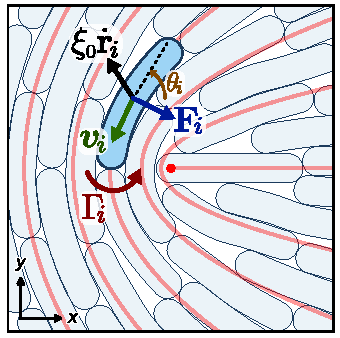
\includegraphics[page=1,height=3.2cm]{media/paper-main}};
  \node[below=1mm of rods,font=\footnotesize] {reversing rods\\ \textit{M.~xanthus}};
  \node[right=of rods,draw=black,very thick,rounded corners=4pt,
        text width=2.5cm,minimum height=2.2cm] (dean)
        {\textbf{Dean's method}\\[1ex]\footnotesize $N$ particles $\to$\\ one field equation};
  \node[right=of dean,draw=litegray,thick,rounded corners=4pt,text width=2.0cm,minimum height=2.2cm] (fields)
        {density $\rho$\\ nematic $\Q$\\[0.5ex] \colN{+ noise}};
  \node[right=of fields] (layer) {\includegraphics[page=2,trim=106 0 243 2,clip,height=3.2cm]{media/paper-main}};
  \node[below=1mm of layer,font=\footnotesize] {new layer};
  \draw[->,very thick] (rods) -- (dean);
  \draw[->,very thick] (dean) -- (fields);
  \draw[->,very thick] (fields) -- (layer);
  \node[below=0.9cm of dean.south east,font=\large,text=darkgreen] {noise \textbf{derived}, not added};
\end{tikzpicture}

\vspace{2ex}
{\small \textbf{hypothesis:} \colN{polarity fluctuations} $\to$ pressure fluctuations $\to$ new layer}

\note{[1:00]
Why this paper? It is the key component of my current project.

We study \textit{Myxococcus xanthus}: rod-shaped bacteria that glide on a surface and reverse their direction of motion, so their polarity flips. In a dense monolayer, cells are sometimes pushed up and start a new layer, as in the microscopy on the right.

Our hypothesis: fluctuations, not the average fields, trigger these layers; polarity fluctuations become pressure fluctuations. So I need field equations that keep the noise of the individual cells.

Dean's method gives exactly that: from the equation of motion of each particle to field equations for the density and the nematic order, with the noise derived, not added by hand. It needs It\^o's lemma and Gaussian white noise, so it carries over to self-propelled rods once their reversals are approximated by white noise.

Today: the original version, passive Brownian particles with pair interactions.}
\end{frame}


% ===========================================================================
% 3. The question
% ===========================================================================
\begin{frame}[t]{The question: from particles to a density field}
\vspace{1ex}
\begin{columns}[t]
\column{0.54\textwidth}
\centering
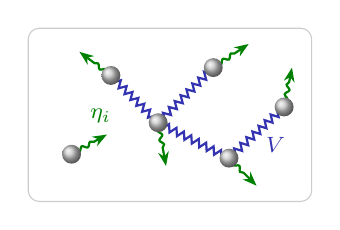
\begin{tikzpicture}[x=1cm,y=1cm]
  \draw[litelitegray,rounded corners] (-0.3,-0.25) rectangle (3.3,1.95);
  \coordinate (P1) at (0.25,0.35); \coordinate (P2) at (0.75,1.35);
  \coordinate (P3) at (1.35,0.75); \coordinate (P4) at (2.05,1.45);
  \coordinate (P5) at (2.25,0.30); \coordinate (P6) at (2.95,0.95);
  \foreach \a/\b in {P2/P3,P3/P4,P3/P5,P5/P6}
    \draw[bblue,thick,decorate,decoration={zigzag,amplitude=1.3pt,segment length=3pt}] (\a) -- (\b);
  \foreach \p/\dx/\dy in {P1/0.45/0.25,P2/-0.4/0.3,P3/0.1/-0.55,P4/0.45/0.3,P5/0.35/-0.35,P6/0.1/0.5}
    \draw[darkgreen,thick,-{Stealth[length=1.8mm]},decorate,
          decoration={snake,amplitude=0.7pt,segment length=3.5pt,post length=1.8mm}] (\p) -- ++(\dx,\dy);
  \foreach \p in {P1,P2,P3,P4,P5,P6} \shade[ball color=gray!45] (\p) circle (0.12);
  \node[font=\footnotesize,text=bblue,anchor=north west,inner sep=1pt] at (2.68,0.6) {$V$};
  \node[font=\footnotesize,text=darkgreen,anchor=south] at (0.62,0.62) {$\eta_i$};
\end{tikzpicture}
\small
\[
\begin{aligned}
  \frac{\d X_i}{\d t} &= \colN{\eta_i(t)} - \colI{\textstyle\sum_{j}\nabla V(X_i-X_j)}\\
  \colN{\la\eta_i^\mu(t)\,\eta_j^\nu(t')\ra} &= 2T\,\delta_{ij}\,\delta^{\mu\nu}\,\delta(t-t')
\end{aligned}\;\eqn{1, 2}
\]
{\footnotesize any $N$, any pair potential $V$, any dimension}

\column{0.06\textwidth}
\vspace{1.0cm}
{\LARGE $\Rightarrow$}

\column{0.40\textwidth}
\centering
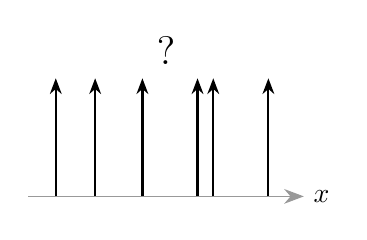
\begin{tikzpicture}[x=1cm,y=1cm]
  \draw[->,litegray] (-0.1,0) -- (3.4,0) node[right,text=black]{$x$};
  \foreach \s in {0.25,0.75,1.35,2.05,2.25,2.95}
    \draw[-{Stealth[length=2mm]},thick] (\s,0) -- (\s,1.5);
  \node[font=\Large] at (1.65,1.85) {?};
\end{tikzpicture}
\small
\[
\begin{aligned}
  \rho_i(x,t) &= \delta\big(X_i(t)-x\big)\\
  \rho(x,t) &= \textstyle\sum_i \rho_i(x,t)
\end{aligned}\;\eqn{3, 4}
\]
{\footnotesize closed equation for $\rho$?}
\end{columns}

\vfill
\onslide<2->{%
\centering\footnotesize
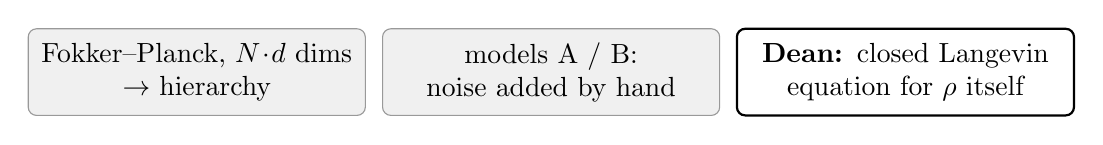
\begin{tikzpicture}[every node/.style={rounded corners=3pt,inner sep=4pt,align=center,text width=4.0cm,minimum height=1.1cm}]
  \node[draw=litegray,fill=litelitegray!30] (fp) at (0,0) {Fokker--Planck, $N\!\cdot\!d$ dims\\ $\to$ hierarchy};
  \node[draw=litegray,fill=litelitegray!30] (ab) at (4.5,0) {models A / B:\\ noise added by hand};
  \node[draw=black,thick] (dn) at (9.0,0) {\textbf{Dean:} closed Langevin\\ equation for $\rho$ itself};
\end{tikzpicture}}

\note{[1:00]
The setting is very general. $N$ overdamped particles, each kicked by its own thermal white noise at temperature $T$ (green), and interacting through an arbitrary pair potential $V$ (blue); Dean mentions Coulomb, Lennard-Jones, even hard spheres. That is eq.~(1).

The density of particle $i$ is a delta function at its position, $\rho_i$; the total density is their sum. Question: is there a closed equation for this field?

\clk Two usual routes. First: the Fokker--Planck equation in the full space, $N$ times $d$ dimensions, then projection operators, and a hierarchy for the $n$-point correlations. Second: phenomenology: write a free energy and add noise by hand, models A and B.

Dean takes a third route: a closed Langevin equation for $\rho$ itself, without averaging over the noise.}
\end{frame}


% ===========================================================================
% 4. Step 1
% ===========================================================================
\begin{frame}[t]{Step 1: one particle}
\small\setlength{\abovedisplayskip}{4pt}\setlength{\belowdisplayskip}{4pt}
\onslide<+->
Test function $\hlf{f}$; a tautology:
\begin{align*}
  f\big(X_i(t)\big) = \int\!\d x\;\rho_i(x,t)\,\hlf{f(x)} \eqtag{5}
\end{align*}
\onslide<+->
It\^o's lemma, then integration by parts:
\begin{align*}
  \frac{\d f(X_i)}{\d t}
  &= \int\!\d x\;\rho_i\Big[
     \colN{\nabla f\cdot\eta_i}
     - \colI{\nabla f\cdot\textstyle\sum_{j}\nabla V(x-X_j)}
     + \lab{\colD{T\,\nabla^2 f}}{It\^o: $\d X\d X\sim 2T\d t$}
     \Big] \eqtag{6}\\
  &= \int\!\d x\;\hlf{f}\,\Big[
     \colN{-\nabla\cdot(\rho_i\,\eta_i)}
     + \colI{\nabla\cdot\big(\rho_i\textstyle\sum_{j}\nabla V(x-X_j)\big)}
     + \colD{T\,\nabla^2\rho_i}
     \Big] \eqtag{7}
\end{align*}
\onslide<+->
Compare with $\displaystyle\frac{\d}{\d t}\!\int\!\d x\,\rho_i\,f=\int\!\d x\,\hlf{f}\,\partial_t\rho_i$ \eqn{8}, for every $f$:
\begin{align*}
  \boxed{\partial_t\rho_i
  = \colN{-\nabla\cdot(\rho_i\,\eta_i)}
  + \colI{\nabla\cdot\big(\rho_i\textstyle\sum_{j}\nabla V(x-X_j)\big)}
  + \colD{T\,\nabla^2\rho_i}} \eqtag{9}
\end{align*}
{\footnotesize\color{darkgreen} no average over the noise yet: one realization}

\onslide<1->
\vfill
\deanlegend
\note{[1:05]
The derivation has two steps. Step one: a single particle.

Take any test function $f$. Evaluating $f$ at the particle position is the same as integrating $f$ against the one-particle density $\rho_i$: eq.~(5), a tautology.

\clk Differentiate $f(X_i)$ with It\^o's lemma. Three terms: noise (green), force from the other particles (blue), and the It\^o term $T\nabla^2 f$ (orange), which comes from the second-order term, because $dX\,dX$ is of order $dt$. Integrate by parts: the derivatives move from $f$ onto $\rho_i$.

\clk Compare with the time derivative of eq.~(5). Since $f$ is arbitrary, we read off the equation for $\rho_i$, eq.~(9).

Dean stresses: the argument is standard; the only subtlety is that nothing has been averaged over the noise.}
\end{frame}


% ===========================================================================
% 5. Step 2
% ===========================================================================
\begin{frame}[t]{Step 2: sum over particles, and the noise trick}
\small\setlength{\abovedisplayskip}{2pt}\setlength{\belowdisplayskip}{2pt}
\onslide<+->
Sum over $i$: \colI{drift closes in $\rho$}, \colN{noise does not}
\begin{align*}
  \partial_t\rho = \colN{\xi} + \colI{\nabla\cdot\Big(\rho\!\int\!\d y\,\rho(y)\,\nabla V(x-y)\Big)} + \colD{T\nabla^2\rho},
  \qquad \colN{\xi = -\textstyle\sum_i\nabla\cdot\big(\eta_i\,\rho_i\big)} \eqtag{10, 11}
\end{align*}
\onslide<+->
Gaussian, given the positions (It\^o): only the correlator matters
\begin{align*}
  \colN{\la\xi(x,t)\,\xi(y,t')\ra} &= 2T\delta(t-t')\textstyle\sum_i\nabla_x\cdot\nabla_y\big[\hlf{\rho_i(x,t)\,\rho_i(y,t)}\big] \eqtag{12}
\end{align*}
\onslide<+->
\textbf{The trick:} one particle, one place:\quad $\mathhlbox{liteyellow}{\rho_i(x,t)\,\rho_i(y,t)=\delta(x-y)\,\rho_i(x,t)}$\hfill\eqn{13}
\begin{align*}
  \colN{\la\xi(x,t)\,\xi(y,t')\ra} = 2T\delta(t-t')\,\nabla_x\cdot\nabla_y\big[\delta(x-y)\,\hlf{\rho(x,t)}\big] \eqtag{14}
\end{align*}
\par\vspace{1ex}
\onslide<+->
\begin{minipage}[c]{0.57\linewidth}
\centering
\begin{tikzpicture}[x=1cm,y=1cm,scale=1.15]
  % N particle noises
  % two clusters, matching the two bumps of the field on the right
  \foreach \px/\py/\dx/\dy in {0.15/0.25/0.3/0.25, 0.45/0.8/-0.3/0.2, 0.75/0.3/0.1/-0.3, 1.55/0.75/0.3/0.15, 1.85/0.25/-0.1/0.35}{
    \draw[darkgreen,thick,-{Stealth[length=1.5mm]},decorate,
          decoration={snake,amplitude=0.5pt,segment length=3pt,post length=1.5mm}] (\px,\py) -- ++(\dx,\dy);
    \shade[ball color=gray!45] (\px,\py) circle (0.09);
  }
  \node[font=\footnotesize,align=center] at (1.05,-0.4) {$N$ noises $\colN{\eta_i(t)}$};
  \node[font=\Large] at (2.75,0.45) {$\Rightarrow$};
  % one noise field: random current along x, amplitude sqrt(rho)
  \begin{scope}[xshift=3.2cm,x=0.72cm,y=0.9cm]
    \fill[litelitegray!60] plot[variable=\t,domain=0:4.2,samples=80] (\t,{rhoprof(\t)}) -- (4.2,0) -- (0,0) -- cycle;
    % one realization: random sign, length = sqrt(rho); none in the gap
    \foreach \t/\s/\h in {0.35/1/0.25,0.6/-1/0.62,0.9/1/0.25,1.2/-1/0.62,1.45/1/0.25,
                          2.65/-1/0.25,2.9/1/0.62,3.15/-1/0.25,3.45/1/0.62}
      \draw[darkgreen,very thick,-{Stealth[length=1.6mm]}] (\t,{\h*rhoprof(\t)}) -- ++({0.5*\s*sqrt(rhoprof(\t))},0);
    \draw[litegray] (0,0) -- (4.3,0);
    \node[font=\scriptsize,text=softgray] at (2.05,0.18) {gap};
    \node[font=\footnotesize,align=center] at (2.1,-0.45) {one field $\colN{\eta(x,t)}$: current $\propto\sqrt{\rho}$};
  \end{scope}
\end{tikzpicture}
\end{minipage}%
\hfill
\begin{minipage}[c]{0.42\linewidth}
same statistics:
\begin{align*}
  &\colN{\xi}\;\to\;\colN{\nabla\cdot\big(\eta(x,t)\,\rho^{1/2}\big)} \eqtag{15}\\[1ex]
  &\colN{\la\eta^\mu(x,t)\,\eta^\nu(y,t')\ra}\\
  &\quad= 2T\delta^{\mu\nu}\delta(x-y)\,\delta(t-t') \eqtag{16}
\end{align*}
\end{minipage}

\onslide<1->
\vfill
\deanlegend

\note{[1:15]
Step two: sum over particles.

The drift closes: the one-particle densities add up to $\rho$, and the sum of forces becomes an integral over $\rho$. The noise $\xi$ does not: it is still a sum over particles, each with its own kick.

\clk Now the noise. Given the positions, $\xi$ is Gaussian, so only its correlator matters. The particle noises are independent, so only $i=j$ survives.

\clk Here is the trick: one particle sits at one place, so $\rho_i(x)\rho_i(y)$ is $\delta(x-y)\rho_i(x)$. Summing over $i$ gives $\rho$: the correlator depends on $\rho$ only.

\clk So replace $\xi$ by any Gaussian noise with this correlator: a new white-noise field $\eta(x,t)$, one for the whole system, times $\sqrt{\rho}$; a random current. It vanishes in the gap. The swap holds in law, not kick by kick: the statistics of $\rho$ stay exact.}
\end{frame}


% ===========================================================================
% 6. Result
% ===========================================================================
\begin{frame}[t]{Dean's equation}
\setlength{\abovedisplayskip}{4pt}\setlength{\belowdisplayskip}{4pt}
\begin{align*}
  \boxed{\partial_t\rho
  = \nabla\cdot\Big(\rho\,\nabla\frac{\delta F}{\delta\rho}\Big)
  + \colN{\nabla\cdot\big(\eta\,\rho^{1/2}\big)}} \tag*{{\footnotesize\color{softgray}It\^o, as derived}\ \eqn{17, 19}}
\end{align*}
\begin{align*}
  F[\rho] = \lab{\colI{\frac12\!\int\!\d x\,\d y\;\rho(x)\,V(x-y)\,\rho(y)}}{interaction energy}
  + \lab{\colD{T\!\int\!\d x\;\rho\log\rho}}{entropy ($-TS$) \color{darkorange}$\to$ It\^o term} \eqtag{18}
\end{align*}

\vspace{1ex}
\onslide<2->{%
{\small Compare with model B (phenomenological, conserved):}
\begin{align*}
  \text{Dean:}\quad   \partial_t\rho &= \nabla\cdot\Big(\underset{\mathclap{\text{\scriptsize mobility}}}{\mathhlbox{liteyellow}{\rho}}\,\nabla\frac{\delta F}{\delta\rho}\Big) + \colN{\nabla\cdot\big(\eta\,\underset{\mathclap{\text{\scriptsize\color{darkgreen}multiplicative}}}{\mathhlbox{litegreen}{\rho^{1/2}}}\big)}\\[1ex]
  \text{model B:}\quad \partial_t\rho &= \nabla\cdot\Big(\mathhlbox{liteyellow}{1}\,\nabla\frac{\delta F}{\delta\rho}\Big) + \colN{\nabla\cdot\big(\eta\,\mathhlbox{litegreen}{1}\big)} \eqtag{23}
\end{align*}}

\note{[0:55]
Together, this is Dean's equation, with the free energy $F$: the pair interaction energy (blue) plus the ideal-gas entropy term $T\int\rho\log\rho$, that is $-TS$ (orange). The entropy is the It\^o term in disguise: $T$ times the Laplacian of $\rho$ is the divergence of $\rho$ times the gradient of $T\log\rho$. Dean does not name a convention for the $\sqrt{\rho}$ noise; his derivation uses It\^o calculus, so $\rho$ is taken before each kick.

\clk Compare with model B, the standard phenomenological equation for a conserved order parameter. Same structure: a conserved current driven by the gradient of $\delta F/\delta\rho$, plus conserved noise. Two differences: the mobility is $\rho$ itself, not a constant; and the noise is multiplicative, $\eta\sqrt{\rho}$.}
\end{frame}


% ===========================================================================
% 7. Properties
% ===========================================================================
\begin{frame}[t]{What comes for free}
\vspace{1ex}
\begin{columns}[t]
\column{0.32\textwidth}
\centering
{\textbf{$N$ is conserved}}\\[2ex]
$\partial_t\rho=\nabla\cdot(\ldots)$\\[1ex]
$\Downarrow$\\[1ex]
$\displaystyle\frac{\d}{\d t}\!\int\!\d x\,\rho = 0$\\[1ex]
{\footnotesize in every realization}

\column{0.34\textwidth}
\centering
{\color{darkgreen}\textbf{no noise where $\rho=0$}}\\[1ex]
\begin{tikzpicture}[x=0.9cm,y=1.1cm]
  \pgfmathsetseed{3}
  \draw[thick,darkgreen] plot[variable=\t,domain=0:4.2,samples=140]
     (\t,{rhoprof(\t)+0.16*sqrt(rhoprof(\t))*(2*rnd-1)});
  \draw[->,litegray] (0,0) -- (4.4,0) node[right,text=black,font=\footnotesize]{$x$};
  \draw[<->,softgray] (1.55,-0.18) -- (2.45,-0.18);
  \node[font=\scriptsize,below] at (2.0,-0.18) {$\rho=0$};
\end{tikzpicture}\\[0.5ex]
{\footnotesize noise $\propto\sqrt{\rho}$}

\column{0.32\textwidth}
\centering
{\color{darkorange}\textbf{Boltzmann, any $N$}}\\[2ex]
$P[\rho]\propto \ee^{-F[\rho]/T}$\\ {\footnotesize (formally)} \eqn{24}\\[1.5ex]
{\footnotesize $T\rho\log\rho$ without coarse-graining\\ or Stirling's formula}
\end{columns}

\vfill
\onslide<2->{%
\centering
\setlength{\fboxsep}{6pt}\fbox{\textbf{Derivation without approximation:} any $N$ $\cdot$ any pair potential $V$ $\cdot$ any $d$}

\vspace{2ex}
{\footnotesize\color{softgray} gain: closed before averaging\quad$\cdot$\quad price: averaging gives back the BBGKY hierarchy
$\la\rho\rho\ra\leftarrow\la\rho\rho\rho\ra\leftarrow\cdots$ \eqn{26}}}

\note{[0:55]
Three properties come for free.

First: everything is a divergence, so the particle number is conserved, in every realization.

Second: the noise is multiplicative. Where there are no particles, the density cannot fluctuate.

Third: $\exp(-F/T)$ is, formally, a stationary solution of the functional Fokker--Planck equation. What surprised me, and Dean comments on it: the entropy $\rho\log\rho$ appears directly, without any appeal to a large number of particles. Usually it comes from coarse-graining plus Stirling's formula.

\clk And no approximation anywhere in the derivation: any $N$, any pair potential, any dimension.

The gain: before averaging, the equation is closed. The price: averaging gives back the dynamical BBGKY hierarchy, eq.~(26), the same as on the Fokker--Planck route. So: exact, but formal. The follow-ups deal with that.}
\end{frame}


% ===========================================================================
% 8. Follow-ups
% ===========================================================================
\begin{frame}[t]{Thirty years of follow-ups}
\begin{wide}{12pt}
\centering
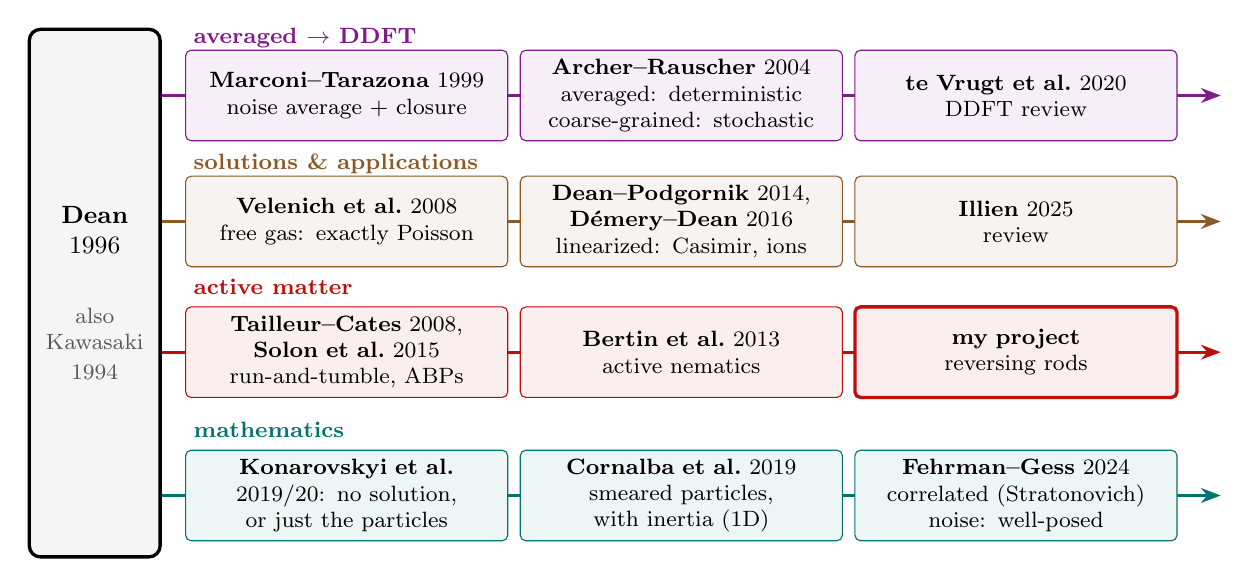
\begin{tikzpicture}[x=1cm,y=1cm]
  % Dean, the root
  \def\yD{2.36}\def\yS{0.76}\def\yA{-0.90}\def\yM{-2.72}
  \node[draw=black,fill=black!4,very thick,rounded corners=4pt,align=center,
        minimum height=6.7cm,text width=1.45cm,font=\small,inner sep=3pt] (dean) at (0,-0.15)
        {\textbf{Dean}\\ 1996\\[4ex]{\footnotesize\color{softgray}also\\ Kawasaki\\ 1994}};
  % lanes: arrow; label sits on the first card (offset = half its height)
  \foreach \yy/\dy/\cc/\name in {\yD/0.60/laneD/averaged $\to$ DDFT, \yS/0.60/laneS/solutions \& applications,
                                 \yA/0.73/laneA/active matter, \yM/0.73/laneM/mathematics}{
    \draw[\cc,very thick,->] (dean.east |- 0,\yy) -- (14.3,\yy);
    \node[lane=\cc,anchor=south west,inner sep=0pt] at (1.25,\yy+\dy) {\name};
  }
  \def\xa{3.2}\def\xb{7.45}\def\xc{11.7}
  % averaged / DDFT
  \begin{scope}[visible on=<2->]
  \node[card=laneD] at (\xa,\yD) {\textbf{Marconi--Tarazona} 1999\\ noise average + closure};
  \node[card=laneD] at (\xb,\yD) {\textbf{Archer--Rauscher} 2004\\ averaged: deterministic\\ coarse-grained: stochastic};
  \node[card=laneD] at (\xc,\yD) {\textbf{te Vrugt et al.}\ 2020\\ DDFT review};
  \end{scope}
  % solutions & applications
  \begin{scope}[visible on=<3->]
  \node[card=laneS] at (\xa,\yS) {\textbf{Velenich et al.}\ 2008\\ free gas: exactly Poisson};
  \node[card=laneS] at (\xb,\yS) {\textbf{Dean--Podgornik} 2014,\\ \textbf{D\'emery--Dean} 2016\\ linearized: Casimir, ions};
  \node[card=laneS] at (\xc,\yS) {\textbf{Illien} 2025\\ review};
  \end{scope}
  % active matter
  \begin{scope}[visible on=<4->]
  \node[card=laneA] at (\xa,\yA) {\textbf{Tailleur--Cates} 2008,\\ \textbf{Solon et al.}\ 2015\\ run-and-tumble, ABPs};
  \node[card=laneA] at (\xb,\yA) {\textbf{Bertin et al.}\ 2013\\ active nematics};
  \node[card=laneA,very thick] at (\xc,\yA) {\textbf{my project}\\ reversing rods};
  \end{scope}
  % mathematics
  \begin{scope}[visible on=<5->]
  \node[card=laneM] at (\xa,\yM) {\textbf{Konarovskyi et al.}\\ 2019/20: no solution,\\ or just the particles};
  \node[card=laneM] at (\xb,\yM) {\textbf{Cornalba et al.}\ 2019\\ smeared particles,\\ with inertia (1D)};
  \node[card=laneM] at (\xc,\yM) {\textbf{Fehrman--Gess} 2024\\ correlated (Stratonovich)\\ noise: well-posed};
  \end{scope}
\end{tikzpicture}
\end{wide}

\note{[0:50]
Thirty years of follow-ups, in four strands.

Today it is usually called the Dean--Kawasaki equation. The reason: in 1994 Kawasaki wrote an equation for the probability of a locally coarse-grained density, assuming local equilibrium. Illien's review calls it, as a limited analogy, the Fokker--Planck counterpart of Dean's equation.

\clk Purple, averaging: this leads to dynamical density functional theory, DDFT. Archer and Rauscher: the averaged density obeys a deterministic equation, a coarse-grained one a stochastic equation.

\clk Brown: the free gas is solved exactly, with Poisson statistics in equilibrium; linearized versions give Casimir forces and electrolyte conductivity.

\clk Red, active matter: run-and-tumble particles, active Brownian particles, active nematics, and my reversing rods.

\clk Teal, mathematics: what does the equation mean? Next slide.}
\end{frame}


% ===========================================================================
% 9. What is rho
% ===========================================================================
\begin{frame}{What is $\rho$ in Dean's equation?}
\begin{wide}{14pt}
\centering
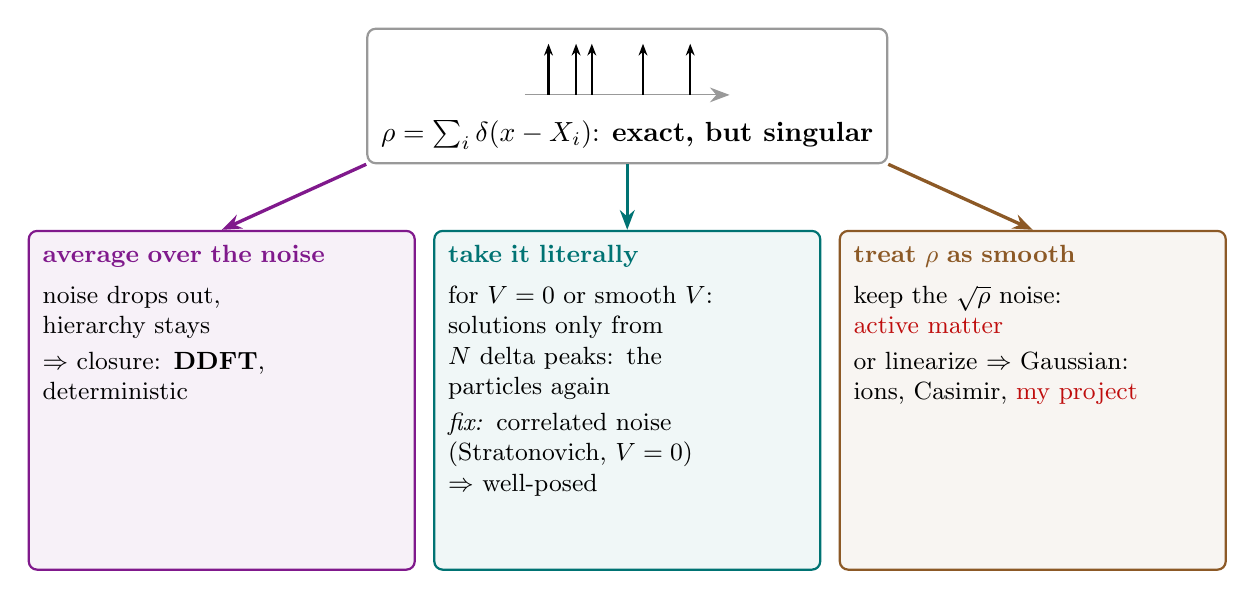
\begin{tikzpicture}[box/.append style={font=\small,text width=4.55cm,minimum height=4.3cm,
    execute at begin node={\vbox to 3.95cm\bgroup},execute at end node={\vfil\egroup}}]
  \node[draw=litegray,thick,rounded corners=3pt,inner sep=5pt,align=center] (rho) at (0,0) {%
    \tikz[x=1cm,y=1cm]{\draw[->,litegray] (0,0) -- (2.6,0);
      \foreach \s in {0.3,0.65,0.85,1.5,2.1}{\draw[-{Stealth[length=1.5mm]},thick] (\s,0) -- (\s,0.65);}}\\[2pt]
    $\rho=\sum_i\delta(x-X_i)$: \textbf{exact, but singular}};
  \node[box=laneD] (avg) at (-5.15,-1.7) {%
    {\color{laneD}\textbf{average over the noise}}\\[1ex]
    noise drops out,\\ hierarchy stays\\[0.5ex]
    $\Rightarrow$ closure: \textbf{DDFT},\\ deterministic};
  \node[box=laneM] (lit) at (0,-1.7) {%
    {\color{laneM}\textbf{take it literally}}\\[1ex]
    for $V=0$ or smooth $V$:\\ solutions only from\\ $N$ delta peaks: the\\ particles again\\[0.5ex]
    \textit{fix:} correlated noise\\ (Stratonovich, $V=0$)\\ $\Rightarrow$ well-posed};
  \node[box=laneS] (smo) at (5.15,-1.7) {%
    {\color{laneS}\textbf{treat $\rho$ as smooth}}\\[1ex]
    keep the $\sqrt{\rho}$ noise:\\ \textcolor{laneA}{active matter}\\[0.5ex]
    or linearize $\Rightarrow$ Gaussian:\\ ions, Casimir, \textcolor{laneA}{my project}};
  \draw[->,very thick,laneD] (rho.south west) -- (avg.north);
  \draw[->,very thick,laneM] (rho.south) -- (lit.north);
  \draw[->,very thick,laneS] (rho.south east) -- (smo.north);
\end{tikzpicture}
\end{wide}

\note{[0:55]
What is $\rho$ in Dean's equation? Exact, but a sum of delta functions. Three ways to live with that.

Left: average over the noise. The noise drops out, the hierarchy stays; an equilibrium closure gives DDFT, deterministic. Adding the noise back would count fluctuations twice.

Middle: take it literally. For free or smoothly interacting particles, Konarovskyi and co-workers proved: solutions exist only from a sum of $N$ delta peaks, and then it is just the particles again. With spatially correlated noise, read in the Stratonovich sense, the equation without pair forces is well-posed (Fehrman and Gess).

Right: treat $\rho$ as a smooth, coarse-grained field. Active-matter theories keep the multiplicative noise; many applications linearize and get Gaussian fluctuations. That is what I do, around a steady state.}
\end{frame}


% ===========================================================================
% 10. Why read it
% ===========================================================================
\begin{frame}[t]{Why you should read it}
\vspace{3ex}
\centering
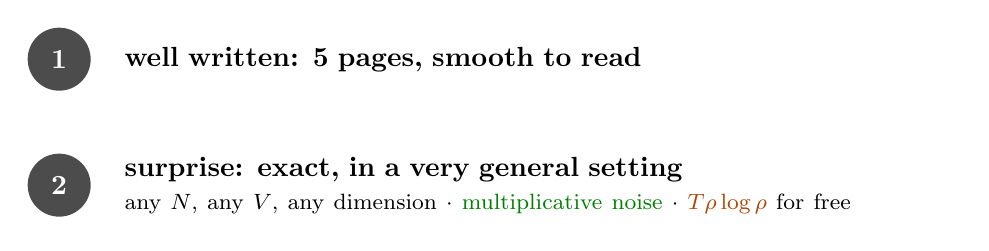
\begin{tikzpicture}[txt/.append style={text width=10.5cm}]
  \node[num=black!70]   (n1) at (0,0)    {1};
  \node[txt] at ($(n1.east)+(0.3,0)$)    {\textbf{well written: 5 pages, smooth to read}};
  \node[num=black!70]   (n2) at (0,-1.6) {2};
  \node[txt] at ($(n2.east)+(0.3,0)$)    {\textbf{surprise: exact, in a very general setting}\\ {\footnotesize any $N$, any $V$, any dimension $\cdot$ \colN{multiplicative noise} $\cdot$ \colD{$T\rho\log\rho$} for free}};
\end{tikzpicture}

\vfill
\centering
{\footnotesize\color{softgray} + thirty years of follow-ups: DDFT, active matter, rigorous mathematics}

\vspace{2ex}
{\large\color{bblue} Thank you}

\note{[0:40]
Why should you read it?

One: it is well written. Five pages; every step is short and explained in words.

Two: the surprise. No approximation (any $N$, any pair potential, any dimension), and still a closed field equation, with multiplicative noise and the free energy appearing by itself.

And it started thirty years of work. Thank you.}
\end{frame}

% ===========================================================================
% References (after "Thank you", not counted in the 10 frames)
% ===========================================================================
\appendix
\begin{frame}[t,plain]{References}
\scriptsize
\begin{columns}[t]
\column{0.5\textwidth}
\textbf{The paper}
\begin{itemize}\setlength{\itemsep}{0pt}
  \item D.\,S.~Dean, J.~Phys.~A: Math.~Gen.~\textbf{29}, L613 (1996)
  \item K.~Kawasaki, Physica A \textbf{208}, 35 (1994)
  \item P.~Illien, Rep.~Prog.~Phys.~\textbf{88}, 086601 (2025) \emph{(review)}
\end{itemize}
\textbf{Averaged $\to$ DDFT}
\begin{itemize}\setlength{\itemsep}{0pt}
  \item U.~Marini Bettolo Marconi, P.~Tarazona, J.~Chem.~Phys.~\textbf{110}, 8032 (1999)
  \item A.\,J.~Archer, M.~Rauscher, J.~Phys.~A: Math.~Gen.~\textbf{37}, 9325 (2004)
  \item M.~te Vrugt, H.~L\"owen, R.~Wittkowski, Adv.~Phys.~\textbf{69}, 121 (2020)
\end{itemize}
\textbf{Solutions \& applications}
\begin{itemize}\setlength{\itemsep}{0pt}
  \item A.~Velenich et al., J.~Phys.~A: Math.~Theor.~\textbf{41}, 235002 (2008)
  \item D.\,S.~Dean, R.~Podgornik, Phys.~Rev.~E \textbf{89}, 032117 (2014)
  \item V.~D\'emery, D.\,S.~Dean, J.~Stat.~Mech.~(2016) 023106
\end{itemize}
\column{0.5\textwidth}
\textbf{Active matter}
\begin{itemize}\setlength{\itemsep}{0pt}
  \item J.~Tailleur, M.\,E.~Cates, Phys.~Rev.~Lett.~\textbf{100}, 218103 (2008)
  \item E.~Bertin et al., New J.~Phys.~\textbf{15}, 085032 (2013)
  \item A.\,P.~Solon, M.\,E.~Cates, J.~Tailleur, Eur.~Phys.~J.~ST \textbf{224}, 1231 (2015)
\end{itemize}
\textbf{Mathematics}
\begin{itemize}\setlength{\itemsep}{0pt}
  \item V.~Konarovskyi, T.~Lehmann, M.-K.~von Renesse, Electron.~Commun.~Probab.~\textbf{24}, 8 (2019); J.~Stat.~Phys.~\textbf{178}, 666 (2020)
  \item F.~Cornalba, T.~Shardlow, J.~Zimmer, SIAM J.~Math.~Anal.~\textbf{51}, 1137 (2019)
  \item B.~Fehrman, B.~Gess, Arch.~Ration.~Mech.~Anal.~\textbf{248}, 20 (2024)
\end{itemize}
\end{columns}
\end{frame}

\end{document}
